\chapter{Revisão Bibliográfica}\label{chap:odometria visual}


Odometria Visual (OV) é um método de estimação da posição através de um fluxo de imagens de uma câmara (Sistema monocular) ou várias câmaras (Sistema estéreo) \cite{Ericson2018}. OV foi durante muitos anos, um dos estudos pioneiros de Nister, Narodistsky and Bergen \cite{Nisterb}. O trabalho deles resultou num algoritmo em que extrai pontos característicos de  uma imagem, cruzavam com outros e , no fim, usavam para obter uma estimativa de movimento. 

A implementação de OV em locais interiores é bem sucedida enquanto que em locais exteriores são notórios alguns problemas. Alguns fatores, como sombras e objetos dinâmicos, causam  dificuldades de localização em locais exteriores. Para OV funcionar eficientemente é necessário iluminação suficiente e ambiente estático para permitir que o movimento seja extraído corretamente. 

OV tem uma ampla aplicação e foi implementada em diferentes campos eficientemente. Os domínios de aplicação incluem robótica e automação. Os tipos de aplicação são sistemas robóticos móveis, tais como terrestre, subaquáticos, aéreos e espaciais.

Em termos terrestres, a OV é usada para a navegação e deteção de objetos eficientemente. Quanto aos sistemas robóticos moveis subaquáticos, a OV tem um papel significativo nos veículos autónomos subaquáticos e sistemas de inspeção de recifes de corais \cite{Aqel2016}. A nível aéreo, a OV é aplicada a \textit{drones} (UAVs) para melhorar a performance de navegação autónoma. Por último, na exploração espacial , a OV é usada para estimar o movimento do robô NASA Mars  \cite{Cheng} .


Na indústria , OV desempenha um papel importante. É aplicada em sistemas de apoio à condução, tal como em sistema de travagem assistida baseados em visão.  Em grande parte dos veículos são utilizados sensores de visão para navegação e deteção de obstáculos devido ao sinal de GPS ser fraco, ser de leve implementação (em veículos pequenos é crucial) e ser suficientemente eficaz para o baixo custo.  Na agricultura é utilizada OV para estimação relativa em relação às culturas \cite{ericson2008visual,Mendes2016}.


\section{Contextualização}

Nesta secção é feito um breve resumo da computação em sistemas de OV.

Com base no artigo \cite{VOpart1}, um determinado agente ligado a um sistema de câmaras move-se num determinado ambiente e captura imagens em instantes de tempo discreto \textit{k}. Caso o sistema seja composto por visão monocular, o conjunto de imagens capturadas em intervalos de \textit{k} é representado por  \textit{$I_{0:n}$}  = \{\textit{$I_0$}, ..., \textit{$I_n$}\}. 
No caso de ter visão estéreo, então existem duas imagens (esquerda e direita) em cada instante de tempo, representadas por \textit{$I_{e,0:n}$} = \{\textit{$I_{e,0}$}, ..., \textit{$I_{e,n}$}\} e \textit{$I_{d,0:n}$} = \{\textit{$I_{d,0}$}, ..., \textit{$I_{d,n}$}\}. 
Na Figura ~\ref{fig:arch} é apresentado uma ilustração deste cenário. 


\begin{figure}[h!] %colocar figura a seguir ao texto anterior
	\begin{center}
		\leavevmode		
		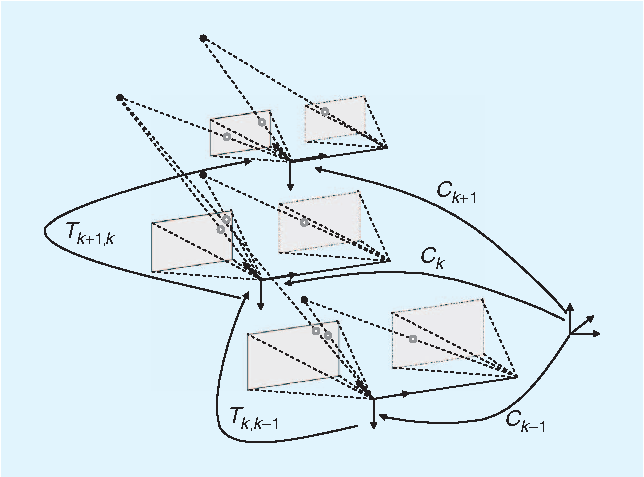
\includegraphics[width=0.65\textwidth]{problVO}
		\caption{Ilustração do problema de OV para visão estéreo.  \cite{VOpart1}}
		\label{fig:arch}
	\end{center}
\end{figure}

Por simplificação, é assumido que o sistema de coordenadas da câmara coincide com o sistema de coordenadas do agente. No caso de sistema estéreo, considera-se que o sistema de coordenadas da câmara esquerda pode ser utilizado como origem sem perda de aspetos gerais.

As posições de uma câmara em instantes de tempo adjacentes \textit{k-1} e \textit{k} estão relacionadas por uma transformação de corpo rígido $T_{k,k-1}$ $\in\ $ $R^{4x4}$ da seguinte forma: \[ T_{k,k-1} = \left[\begin{array}{cc} R_{k,k-1} & t_{k,k-1} \\  0 & 1 \\ \end{array} \right] \]
onde $R_{k,k-1}$ $\in$ $R^{3x3}$ é a matriz de rotação e $t_{k,k-1}$ $\in$ $R^{3x1}$ é o vetor de translação. O conjunto $T_{1:n}$ = \{ $T_{1,0}$, ..., $T_{n,n-1}$ \} contém todos os movimentos sequenciais da câmara. Para simplificar
a notação, a partir de agora, $T_k$ será usado em vez de $T_{k,k-1}$. Finalmente, o conjunto das posições da câmara $C_{0:n}$ = \{ $C_0$, ..., $C_n$ \} contém as transformações da câmara em relação à coordenada da frame inicial no instante \textit{k} = 0. A posição atual $C_n$ pode ser calculada juntando todas a transformações $T_k$ ( \textit{k} = 1 ... n\ ), e assim, $C_n$ = $C_{n-1}T_n$, com $C_0$ sendo a posição da câmara no instante \textit{k} = 0, que pode ser definida arbitrariamente pelo utilizador.

A principal tarefa em um sistema OV é calcular a transformação relativa $T_k$ a partir das imagens $I_k$ e $I_{k-1}$, e depois juntar as transformações para recuperar a trajetória completa $C_{0:n}$ da câmara. Isto significa que o sistema consegue recuperar de forma incremental a trajetória, posição após posição.

A fim de efetuar um sistema de OV é necessário realizar várias etapas. A Figura ~\ref{fig:etapVO} ilustra um diagrama de blocos com a metodologia a utilizar.

\begin{figure}[h!] %colocar figura a seguir ao texto anterior
	\begin{center}
		\leavevmode		
		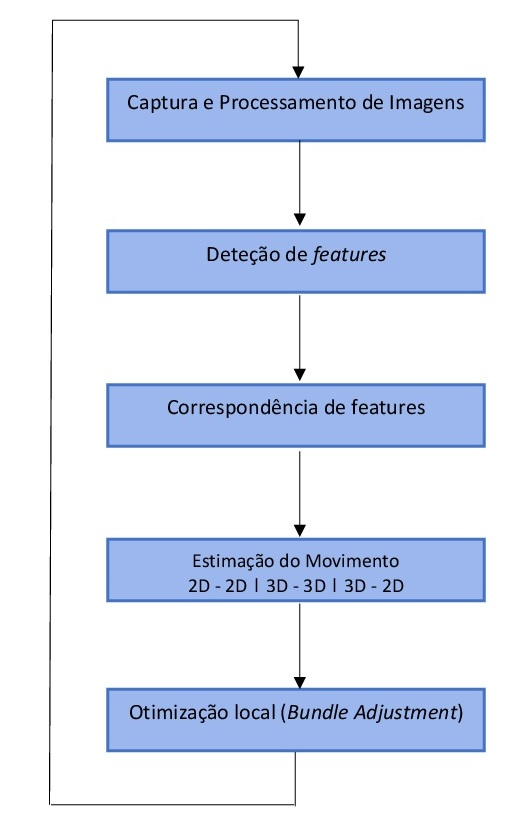
\includegraphics[width=0.4\textwidth]{etapVO}
		\caption{Etapas de um sistema de Odometria Visual.}
		\label{fig:etapVO}
	\end{center}
\end{figure}

Desta forma, a primeira etapa ilustra o processo de captura de uma nova imagem \textit{$I_k$}, ou um par de imagens no caso de um sistema estéreo. Nesta mesma etapa é necessário o processamento da imagem para remover possíveis deformações das imagens ou efeitos de lentes.

A segunda etapa apresenta dois métodos diferentes para encontrar características \footnote{é uma região na imagem que difere da sua vizinhança em termos de intensidade, cor e textura.}, que consistem na procura de características visuais salientes que possam corresponder noutras imagens.

A terceira etapa apresenta dois métodos diferentes para correlacionar características. Nesta mesma etapa são aplicados algoritmos de correção  para remover eventuais erros de correspondência. Uma solução para o problema é a utilização do algoritmo RANSAC.

A quarta etapa consiste no cálculo do movimento relativo $T_k$ entre os instantes de tempo \textit{k} - 1 e \textit{k}. Após a obtenção do $T_k$ então é possível calcular a posição da câmara $C_k$ por junção do $T_k$ com a posição anterior $C_{k-1}$.

Finalmente, a última etapa descreve a aplicação do algoritmo de otimização local, \textit{Buldle Adjustment} , ao longo das últimas características com o objetivo de obter uma estimativa mais precisa da trajetória local.


\section{Parâmetros Intrínsecos}

A formação de uma imagem em uma câmara ocorre com a entrada de feixes de luz através de uma abertura na câmara e a projeção desses feixes em uma tela, também chamada de plano de imagem.

Em uma câmara real, um ponto no mundo reflete diversos feixes de luz. Se todos os feixes refletidos por esse ponto convergirem para um mesmo ponto no plano de imagem, então é dito que a imagem está focada. O modelo de projeção perspetiva é uma simplificação da câmara real.

O modelo de projeção perspetiva é apresentado na Figura ~\ref{fig:modelcamera}. O centro de projecção \textbf{O} é a origem do sistema de coordenadas da câmara e também o centro da câmara. O eixo-z do sistema de coordenadas da câmara é chamado eixo-principal. O plano \textit{z} = \textit{f} é o plano de imagem e a intersecção do plano de imagem com o eixo-principal é chamado ponto principal. Considere $\textbf{X} = [X,Y,Z]^T$ as coordenadas de um ponto no mundo referentes ao sistema de coordenadas da câmara. A intersecção do plano de imagem com o segmento de reta ligando \textbf{X} e \textbf{O} é a projeção de \textbf{X} e é referenciada como \textbf{x}. Por semelhança de triângulos observa-se que \textbf{x} = $[\textit{f} \frac{X}{Z} , \textit{f} \frac{Y}{Z} , \textit{f}]$ em relação à câmara. Como a última coordenada de \textbf{x} será sempre \textit{f}, ela será desconsiderada nas equações daqui em diante.

\begin{figure}[h!]  %colocar figura a seguir ao texto anterior
	\centering
	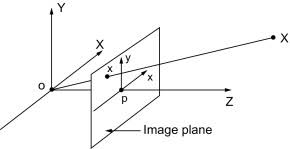
\includegraphics[width=0.6\linewidth]{figures/pinholemodel} 
	\caption{Esquema do modelo de projeção perspetiva. \cite{Yousif2015}}
	\label{fig:modelcamera}  %30 years. Figure 3 a)
\end{figure}

Assim, o mapeamento do mundo 3-D para uma imagem 2-D é obtido através da equação de projeção perspetiva :
\[  \textbf{$\lambda$} \left[ \begin{array}{c} u\\v\\1\\ \end{array} \right] = 
KX = \left[ \begin{array}{ccc} \alpha_u  & 0 & \textit{u}_0 \\ 
0 & \alpha_v & \textit{v}_0 \\ 
0 & 0 & 1 \\
\end{array} \right] \left[ \begin{array}{c} X \\ 
Y \\ 
Z \\ 
\end{array} \right] , \]
onde $\lambda$ é o facto de profundidade, $\alpha_u$ e $\alpha_v$ são as distâncias focais, e $\textit{u}_0$ e $\textit{v}_0$ são as coordenadas centrais da projeção da imagem. Estes parâmetros são conhecidos como parâmetros intrínsecos que dependem de câmara para câmara. Quando o campo de visão da câmara é superior a 45º , os efeitos da distorção radial são visíveis e causam erros superiores.

Note que a última coordenada \textit{w} é a escala da coordenada homogénea e não a distância focal f, que como já foi dito, é desconsiderada daqui em diante. Daqui em diante as coordenadas homogéneas serão representadas por \textbf{x} e \textbf{X} 


\subsection{Lente olho de peixe}

Em câmaras com lentes olho de peixe os parâmetros intrínsecos são diferentes. Estes tipos de lentes são similares à visão humana, onde a imagem resultante tem grande resolução central e baixa resolução nos pontos mais distantes do centro. O modelo mais comum de lentes olho de peixe é o modelo equiangular ,  \[ r = k \theta ,  \] onde k é uma constante \cite{Hansen2009}.

\begin{figure}[h!] %colocar figura a seguir ao texto anterior
	\begin{center}
		\leavevmode		
		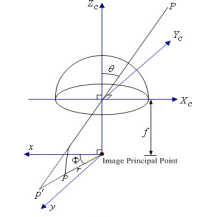
\includegraphics[width=0.4\textwidth]{fisheyemodel}
		\caption{Projeção de um ponto no mundo no plano de imagem. Onde o ponto p' representa projeção perspetiva e o ponto p com o modelo equiangular com distorção da lente olho de peixe. \cite{Srestasathiern2014,Kannala2004}}
		\label{fig:fishvspinhole} 
	\end{center}
\end{figure}

A Figura ~\ref{fig:fishvspinhole} representa a diferença entre a representação de um ponto \textit{P} na imagem captura . Desta forma, o ponto \textit{p'} usa o modelo da projeção perspetiva e o ponto \textit{p} o modelo equiangular onde se visualiza a distorção da lente olho de peixe.

Assim, o algoritmo é descrito pela Figura ~\ref{fig:fisheyealgortim}

\begin{figure}[h!]
	\centering
	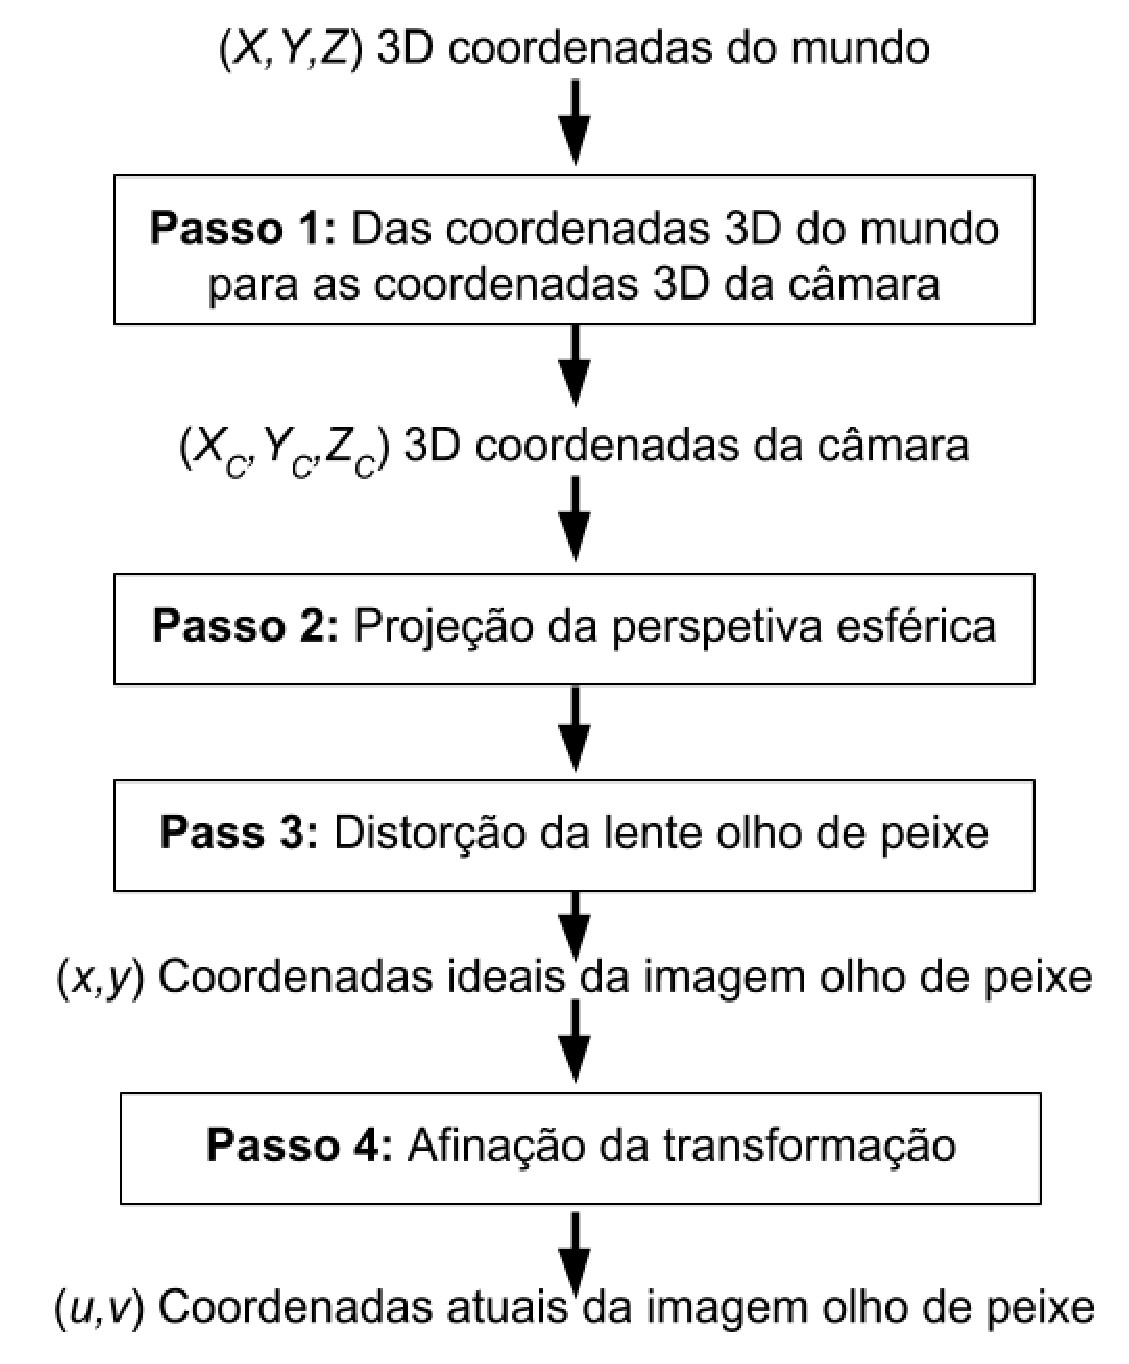
\includegraphics[width=0.4\linewidth]{figures/fisheyealgortimpt}
	\caption{Algoritmo de construção da imagem com lente olho de peixe. \cite{Ying2006}}
	\label{fig:fisheyealgortim}
\end{figure}

Passo 1:  \[ \textbf{P}_\textbf{C} = \textbf{R}\textbf{P}_\textbf{W} + \textbf{t} , \] onde $\textbf{P}_\textbf{C}$ é o ponto capturado na imagem, $\textbf{P}_\textbf{W}$ é o ponto no mundo, \textbf{R} é a matriz de orientação e \textbf{t} é o vetor da posição. Os parâmetros \textbf{R} e \textbf{t} são parâmetros extrínsecos. 

Passo 2: O ponto $\textbf{P}_\textbf{C}$ é projetado com perspetiva de uma esfera resultando o ponto \textbf{p} \[ \textbf{p = $\frac{\textbf{P}_\textbf{C}}{ \| \textbf{P}_\textbf{C} \| }$ } = ( sin \phi cos \theta, sin \phi sin \theta, cos \phi)^T  . \]

Passo 3: O ponto \textbf{p} é mapeado para m no plano de imagem com distorção da lente da câmara \[ m = D(p) , \] onde m = (x,y) e D é o modelo de distorção da lente olho de peixe. 

Passo 4: O ponto m é transformado em m' usando a transformação de afinidade: \[ m' = K_A(m) , \] onde m' = (u,v). A imagem obtida é a imagem atual da câmara com lente olho de peixe que é igual : \[ \widetilde{m}'\ ' = K_A \widetilde{m}'\  ,\] onde $\widetilde{m}'\ $ = $(x,y,1)^T$ e $\widetilde{m}'\ '$ = $(u,v,1)^T$ e $K_A$ =$\left[ \begin{array}{ccc}
r & s & u_0 \\ 
0 & 1 & v_0 \\ 
0 & 0 & 1
\end{array} \right]$ 


Desta forma, concluímos que existem 12 parâmetros para as lentes olho de peixe: 4 parâmetros de transformação de afinidade, 4 radiais e 4 parâmetros de distorção tangencial. Estes parâmetros são os parâmetros intrínsecos das lentes olho de peixe.




\section{Parâmetros Extrínsecos}

Em geral os pontos do mundo são descritos em relação a um sistema de coordenadas global. A relação entre os dois sistemas é dada por uma transformação de corpo rígido do tipo

\[ \textbf{X} = \textbf{R}\textbf{X}_\textbf{W} + \textbf{T},  \]

onde $\textbf{X}_\textbf{W}$ são as coordenadas do ponto \textbf{X} em relação ao sistema de coordenadas global. A matriz \textit{R} $\in$ \textit{$SO(3)$} é a rotação que alinha o sistema de coordenadas global com o sistema de coordenadas da câmara e $\textbf{T}$ $\in$ $\mathbf{R^3}$ é o vetor de translação entre os dois sistemas de coordenadas. Os parâmetros de \textit{R} e \textbf{T} são chamados de parâmetros extrínsecos e a matriz 

\[ [\textit{R}|\textbf{T}] = \left[ \begin{array}{cccc}
r_{11} & r_{12} & r_{13} & t_1 \\ 
r_{21} & r_{22} & r_{23} & t_2 \\ 
r_{31} & r_{32} & r_{33} & t_3
\end{array} \right] \]

é a matriz de parâmetros extrínsecos. A Figura ~\ref{fig:parExt} mostra a relação entre os dois sistemas de coordenadas.

\begin{figure}[h!]
	\centering
	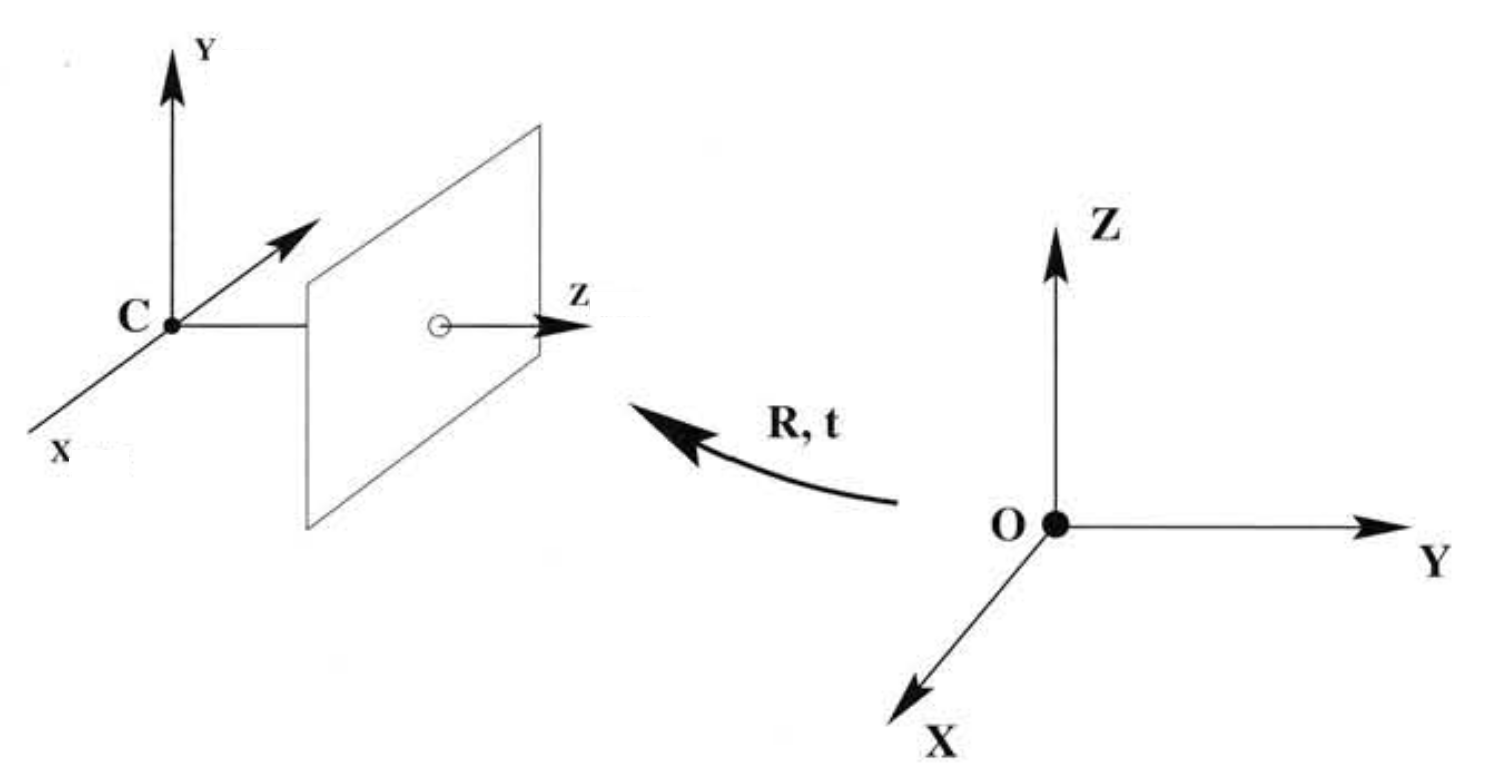
\includegraphics[width=0.7\linewidth]{figures/parExt}
	\caption{Parâmetros que definem a posição e orientação do sistema de coordenadas da câmara com um sistema de coordenadas global.}
	\label{fig:parExt}
\end{figure}


\section{Detetores de Características}\label{detCar}

A deteção de características é o processo responsável por determinar características numa imagem. Uma característica pode ser uma região de uma cor específica, um determinado padrão na imagem, um ponto onde ocorre a variação de cores ou outra informação que possa ser extraída da imagem. Estas características devem ser escolhidas de forma a serem possíveis de encontrar e recuperar futuramente. 

Relativamente a sistemas de OV, foi descoberto que a distribuição de características numa imagem afeta de uma forma considerável os resultados obtidos. Em particular, quanto mais características encontradas mais estáveis são os resultados da estimação do movimento, mas o tempo de processamento é maior e pode causar perdas de \textit{frames} importantes. As características são procuradas numa imagem através de um detetor de características. Para ser um bom detetor de características têm de obedecer às seguintes características \cite{Fraundorfer2012}:
\begin{itemize}
	\item Precisão na localização, tanto em posição como em escala.
	\item Repetibilidade, garante que uma grande percentagem das caracteristicas visíveis a duas imagens serão identificadas em ambas as imagens.
	\item Eficiência computacional, está relacionada ao tempo que o algoritmo de deteção necessita para identificar as características de uma imagem.
	\item Robustez ao ruído e desfocagem
	\item Distinção , de modo que as características possam ser correspondidas precisamente entre imagens diferentes.
	\item Invariância à iluminação e mudanças geométricas, garante que a característica será identificada igualmente com ou sem a transformação.
\end{itemize}

Na área de OV os detetores de características, tais como \textit{cantos}\footnote{é definido como um ponto de intersecção de duas ou mais arestas.} ou \textit{blobs}\footnote{são regiões mais brilhantes (ou mais escuras) do que o meio circundante.}, são muito importantes porque é possível saber com precisão a sua posição numa imagem. 

Entre estes dois tipos de detetores, os detetores de canto são computacionalmente mais rápidos mas menos distintos. Adicionalmente, detetores de canto estão melhores localizados em posições de imagens mas são menos localizados em escala. Isto significa que os detetores de canto podem não ser tão bem detetados que os detetores de \textit{blob} quando existem grandes variações de escala e pontos visíveis. Contudo, detetores de \textit{blob} não são bons em certos ambientes \cite{Fraundorfer2012}.

\subsection{Detetores de Cantos}

Um canto em uma imagem é o ponto onde há uma grande variação de intensidade dos \textit{pixels} em duas direções dominantes. 

\subsubsection{Harris}

O detetor de cantos Harris é um dos métodos mais recentes (1988). A ideia base no algoritmo de Harris é analisar um ponto através das características e de uma pequena vizinhança. Através da alteração da janela em várias direções do ponto , a média da intensidade da janela deve alterar significativamente se o ponto for um canto. Os cenários possíveis são ilustrados na Figura ~\ref{fig:harriscornerdetection}

\begin{figure}[h!]
	\centering
	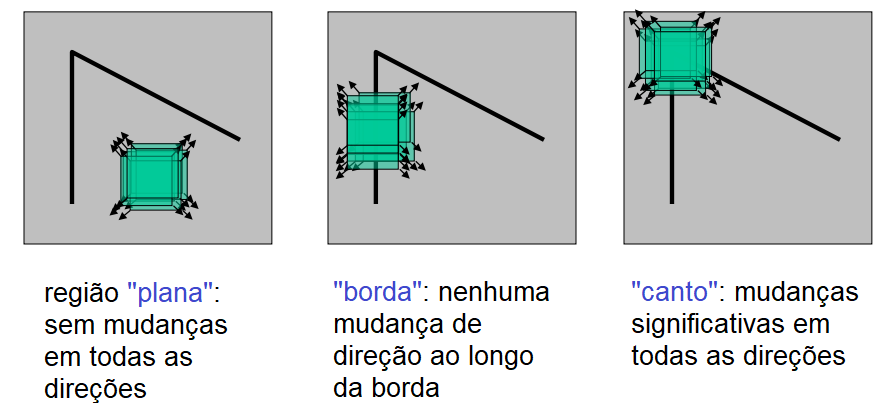
\includegraphics[width=0.7\linewidth]{figures/HarrisCornerDetection}
	\caption{Detetor de cantos Harris. \cite{VisualOdometryRodasVehicles}}
	\label{fig:harriscornerdetection}
\end{figure}

Desde que a janela seja alterada em várias direções , o algoritmo deve obter o mesmo resultado mesmo que a imagem tenha sofrido uma rotação. O mesmo não acontece caso a imagem sofra um zoom , o algoritmo não fornece os mesmos resultados que a imagem original. Assim, o algoritmo é não-invariante à escala. Além de ser computacionalmente pesado no calculo da média da intensidade da janela. %It's also computacionally demanding due to many calculations of the window intesity average. 


\subsubsection{FAST}\label{fastsection}

O detetor de canto FAST (do inglês ,\textit{ Feature from Accelerated Segment Test}) é um detetor rápido. O algoritmo usa um circulo de 16 pixels com um raio de 3 pixels em volta do pixel \textit{p} , de forma a detetar se \textit{p} é um canto, ver Figura ~\ref{fig:fastcornerdetector}.

\begin{figure}[h!]
	\centering
	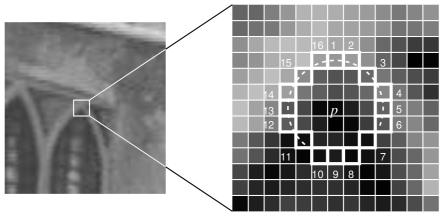
\includegraphics[width=0.7\linewidth]{figures/FASTcornerdetector}
	\caption{Detetor de canto FAST, circulo em volta do ponto \textit{p}. \cite{VisualOdometryRodasVehicles}}
	\label{fig:fastcornerdetector}
\end{figure}

Analisando a Figura  ~\ref{fig:fastcornerdetector} , os pixeis 11-16 e 1-6 têm maior intensidade que os pixel a examinar, pixel \textit{p}. Isto significa que o pixel \textit{p} é um canto. O teste realizado pode ser resumido a duas condições:
\begin{enumerate}
	\item Se existirem N pixeis adjacentes no anel na qual todos têm intensidade superior ao pixel \textit{p}, então \textit{p} é um canto.
	\item Se existirem N pixeis adjacentes no anel na qual todos têm intensidade inferior ao pixel \textit{p}, então \textit{p} é um canto.	
\end{enumerate}
Assim se alguma condição for verdadeira , o pixel \textit{p} é classificado como canto. O parâmetro N é usualmente 12 de forma a obter uma deteção com alta qualidade. N pode ser 9 de forma a detenção ser mais rápida. 
O algoritmo depende da intensidade de threshold , o qual em diferentes ambientes deve originar diferentes resultados e o threshold deve ser ajustado para a melhor performance. Desde que o algoritmo use um círculo de pixeis para determinar se o pixel examinado é um canto, o algoritmo é invariante à escala e rotação.


\subsection{Detectores de blobs}

\subsubsection{SIFT}

A diferença de gaussianas (DoG, do inglês \textit{Diference of Gaussians}) foi utilizada para identificar características invariantes à escala, rotação e parcialmente invariantes à variação na luminosidade e transformações afins. O método SIFT (do inglês, \textit{Scale Invariant Feature Transform}) é composto por um detetor de blobs baseado em DoG.

O primeiro passo no algoritmo de SIFT é utilizar a função gaussiana sobre uma imagem com escalas diferentes para gerar o espaço de escalas da imagem.

A função \begin{equation}\label{equaSIFTdet}
\textit{L}(x,y,\sigma) = \textit{G}(x,y,\sigma)*\textit{I}_{x,y} \end{equation}
define o espaço de escalas da imagem $\textit{I}_{x,y}$. Na equação ~\ref{equaSIFTdet}
, o operador * define a convolução da função gaussiana onde $\textit{I}_{x,y}$ é a imagem de entrada e o núcleo Gaussiano $\textit{G}(x,y,\sigma)$ é igual a  \[ G( \textit{x},\textit{y},\textit{$\sigma$}) =\ \frac{1}{2\pi\sigma^2} e^{-\frac{x^2 + y^2}{2\sigma^2}} . \]

O passo é repetido com diferentes $\sigma$, escalados por um fator $\textit{k}$. \[ \textit{D}(x,y,\sigma) = \textit{L}(x,y,\textit{k}\sigma) - \textit{L}(x,y,\sigma). \]

Desde que todas as DoG estão calculadas para a escala corrente , designada como oitava, a imagem cujo valor de $\sigma$ é duas vezes o valor de $\sigma$ inicial na oitava é selecionada para ser reproduzida. O processo é ilustrado na Figura ~\ref{fig:compitation-of-dog}.

\begin{figure}[h!]
	\centering
	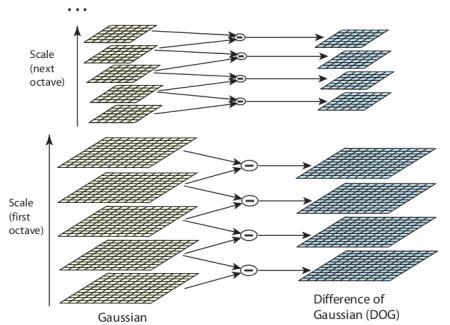
\includegraphics[width=0.7\linewidth]{figures/compitationofDoG}
	\caption{Computação da DoG. \cite{VisualOdometryRodasVehicles}}
	\label{fig:compitation-of-dog}
\end{figure}

Calculadas as DoGs, deseja-se obter os máximos e mínimos locais em todas as escalas de $\textit{D}(x,y,\sigma)$. Para isso avalia-se cada ponto da primeira oitava com seus 26 vizinhos, 8 no mesmo nível e 9 nos níveis superiores e inferiores de escala. A Figura ~\ref{fig:pixelcamadas} apresenta essa comparação. Se o ponto for extremo nessa oitava, sua posição é estimada na oitava seguinte e o processo é repetido para esse ponto. As informações referentes à escala e oitava alcançadas são guardadas e farão parte da característica. 


\begin{figure}[h!]
	\centering
	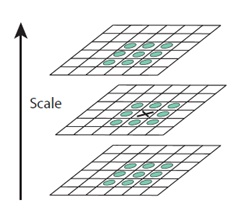
\includegraphics[width=0.5\linewidth]{figures/pixelCamadas}
	\caption{O \textit{pixel} marcado com um \textit{x} é avaliado em relação aos seus vizinhos no mesmo nível e nos níveis superiores e inferiores. \cite{VisualOdometryRodasVehicles}}
	\label{fig:pixelcamadas}
\end{figure}

Uma vez obtido o ponto de extremo é refinada a posição para obter uma posição em $\textit{subpixeis}$. è utilizada uma expansão de Taylor em torno do ponto de extremo \begin{equation}\label{equacao2.1}
D(x) = D + \frac{\partial D^T}{\partial x}x + \frac{1}{2}x^T\frac{\partial^2D}{\partial x^2}x
\end{equation} onde c é o deslocamento em torno do ponto de extremo. O ponto extremo $\hat{x}$ é determinado derivando a equação ~\ref{equacao2.1} em relação a x e igualando a zero. O resultado é dado por \begin{equation}\label{equacao2.2}
\hat{x} = -\frac{\partial^2D^{-1}}{\partial^2x^2}\frac{\partial D}{\partial x}. 
\end{equation} 
Se houver variação maior que 0.5 em qualquer uma das direções o ponto muda de pixel e o valor de extremo é interpolado no novo ponto. O valor do ponto de extremo é refinado para remover extremos com baixo contraste. Essa operação é feita substituindo a equação ~\ref{equacao2.2} na equação ~\ref{equacao2.1}, resultando em \[ D( \hat{x} ) = D + \frac{1}{2}\frac{\partial D^T}{\partial x} \hat{x} . \]

Outro filtro usa uma ideia semelhante para remover pontos de borda. A matriz hessiana \[ \textit{H} = \left[ \begin{array}{cc}
D_{xx} & D_{xy} \\ 
D_{xy} & D_{yy}
\end{array} \right]  \] descreve a curvatura principal da imagem em torno do ponto de extremo. Analisando a relação entre os autovalores de $\textit{H}$ avalia-se que se o determinante de \textit{H} é negativo o ponto é descartado. Assim a avaliação é feita sobre a relação dos autovalores, como mostra a seguinte equação: \begin{equation}\label{equacaoseg}
\frac{\textit{Tr}(H)^2}{\textit{Det}(H)} = \frac{(\alpha + \beta)^2}{\alpha\beta} = \frac{(r\beta + \beta)^2}{r\beta^2} = \frac{(r + 1)^2}{r}, 
\end{equation} 
onde $\alpha$ = $r\beta$. Um valor extremo será descartado caso a relação \[ \frac{\textit{Tr}(H)^2}{\textit{Det}(H)} < \frac{(\tau + 1)^2}{\tau}, \] para um limiar $\tau$ a ser definido.  

Até este ponto foram obtidas localizações e escalas dos pontos de extremos e foram removidos extremos com baixo contraste e em bordas. Resta obter uma orientação para o ponto. Para isso escolhe-se em cada oitava a imagem gaussiana \textit{L} cuja escala mais se aproxima da escala do ponto de extremo. Para cada uma das imagens $\textit{L}(x,y)$  (note que o valor de $\sigma$ não aparece pois é definido como o mesmo do ponto de extremo) a magnitude $\textit{m}(x,y)$ e a orientação $\theta$(x,y) são calculadas usando \[ \textit{m}(x,y) = \sqrt{(\textit{L}(x  +1,y) - \textit{L}(x - 1,y))^2 + (\textit{L}(x,y + 1) - \textit{L}(x,y - 1))^2} \] \[ \theta (x,y) = \textit{tan}^{-1}((\textit{L}(x,y +1) - \textit{L}(x,y - 1))/(\textit{L}(x + 1,y) - \textit{L}(x - 1,y))).\]
Calcula-se as orientações em torno do ponto de extremo e um histograma é montado com 36 orientações possíveis para a característica, cada um respondendo por 10º dos 360º possíveis para $\theta$(x,y). Cada uma das orientações $\theta$(x,y) é pesada utilizando a magnitude $\textit{m}(x,y)$ e uma janela gaussiana com $\sigma$ sendo 1.5 vezes a escala do ponto de extremo antes de ser adicionada à orientação da característica.

Picos no histograma das orientações em torno do ponto de extremo correspondem a direções dominantes do gradiente local. O maior pico de histograma é identificado e uma característica é gerada com localização, escala a e orientação. Picos no histograma que sejam máximos locais e cuja magnitude seja maior que 80\% da do pico máximo também geram características com a mesma localização e escala, mas com a orientação diferente. Por fim, para cada pico que gerou uma característica, uma parábola é traçada pelo pico e os dois valores do histograma adjacentes a ele. Para se obter maior precisão o pico máximo é então tomado como o máximo da parábola gerada pela interpolação dos três picos.


\subsubsection{SURF}

O detetor SURF (do inglês, \textit{Speeded Up Robust Features}) é similar ao SIFT no sentido que os passos são iguais, mas são feitos diferentemente. A imagem em analise é filtrada com janelas baseada no método do integral da imagem, como uma aproximação Gaussiana \begin{equation}\label{surfequation}
I_{\Sigma}(x,y) = \sum_{i}^{x}\sum_{j}^{y}{I(i,j)}. \end{equation}
O benefício do uso deste método é a redução do numero de cálculos e a diferença no tamanho da janela que influenciam no tempo de cálculos. Uma adição e duas subtrações usando os pontos de canto são requeridas para o calculo da soma, Figura ~\ref{fig:surfsqware}.

\begin{figure}[h!]
	\centering
	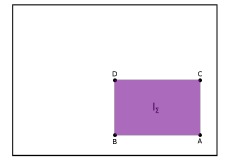
\includegraphics[width=0.4\linewidth]{figures/surfsqware}
	\caption{Ilustração do método do integral da imagem. \cite{VisualOdometryRodasVehicles}}
	\label{fig:surfsqware}
\end{figure}

A soma de todos os pixeis como visto em ~\ref{surfequation} é igual a \textit{$I_{\sum}$} = A - B - C + D, dado que a origem da imagem original é no canto superior esquerdo. Deteção blob é usado e é realizada usando a matriz Hessian. Através de uma imagem \textit{I} e um ponto \textbf{x} = (x,y) na imagem, a matriz Hessian $\textit{H}(x,\sigma)$ é calculada. Onde $\sigma$ é a escala atual. \[  \textit{H}(x,\sigma) = \left[ \begin{array}{cc}
L_{xx}(x,\sigma) & L_{xy}(x,\sigma) \\ 
L_{xy}(x,\sigma) & L_{yy}(x,\sigma)
\end{array} \right]. \] 
Onde $\textit{L}_{xx,xy,yy}(x,\sigma)$  são as derivadas de segunda ordem no ponto x da imagem \textit{I}. Estas derivadas parciais são aproximadas usando filtros para diferentes escalas e oitavas. Depois de suavizar e reduzir a amostragem da imagem para cada $\sigma$ como no algoritmo SIFT, o algoritmo SURF aumenta o tamanho do filtro. Uma vez que o Hessian é formado para o ponto \textbf{x} numa certa escala $\sigma$, o determinante do Hessian é calculado e ponderado de forma a obter a melhor aproximação.  O determinante aproximado é guardado em um mapa de resposta para a escala atual.
Uma vez calculada a matriz Hessian para todas as oitavas, o algoritmo procura o máximo local e o máximo detetado é guardado e interpolado na escala e no espaço da imagem. 

Assim, o detetor de SURF têm pontos chaves:
\begin{itemize}
	\item Localização
	\item Escala
	\item Orientação
\end{itemize}


\section{Descritor de Características}

Como mencionado anteriormente, uma boa característica tem como propriedade a diferenciabilidade. A diferenciabilidade permite que a característica seja identificada de maneira única. Porém se for utilizado somente o ponto de interesse onde localiza-se a característica, a diferenciação torna-se difícil, uma vez que existe pouca informação para gerar um identificador para aquele ponto.

Desta forma, os descritores codificam uma área da imagem em torno do ponto característico, para cada ponto característico. Ao fazer isto, os pontos característicos entre duas imagens são comparáveis uns com os outros.


\subsection{ORB}

O descritor ORB (do inglês, \textit{Oriented FAST and Rotation-Aware BRIEF}) precisa de pontos característicos para serem detetados pelo detetor oFAST. A deteção é realizada como descrita na secção ~\ref{fastsection} com a adição da orientação do ponto característico. Isto é realizado calculando o centroide de intensidade. Primeiro, o momento do patch é calculado como \[ \textit{$m_{pq}$} = \sigma \textit{$ x^py^qI$}(x,y) ,\]
onde \textit{p} e \textit{q} são parâmetros dos pixeis em ordem do momento. E o centroide do patch é encontrado com a seguinte equação \[ C = ( \frac{ \textit{m}_{10} }{ \textit{m}_{00}} ,  \frac{ \textit{m}_{01} }{ \textit{m}_{00}} ) . \]
Em seguida o vetor $\vec{OC}$ é construido do ponto central do ponto de característica, O, para o centroide obtido anteriormente, C. O ângulo de $\vec{OC}$ é obtido com a orientação do patch. \[ \theta = atan^2( \textit{m}_{01},\textit{m}_{10}) . \]
Uma vez atribuída uma orientação ao ponto característico, o descritor BRIEF (do inglês, \textit{Binary Robust Independent Elementary Features}) realiza um teste binário, $\tau$, da intensidade entre pontos de um patch de imagem suavizada. O teste é definido como  \[\sigma\left(p;x,y\right) = \left\{\begin{array}{cc}
1, & p(x)<p(y) \\ 
0, & p(x) \geq  p(y)   
\end{array}\right.
,\]
onde \textbf{p} é o patch de imagem que foi suavizada e \textbf{$(x,y)$} é o ponto de teste.
O resultado da característica é um vetor de 256 testes binários \[ f_{256} \left( p \right) = \sum_{1\ \le\ i\ \le\ 256\ } {2^{i-1}\tau\left(p;x_i,y_i\right) } . \]

De forma a realizar um descritor de recurso elementares independentes robustos binários (BRIEF) invariantes à rotação, é orientar o descritor para a orientação $\theta$ dos pontos caraterísticos. Isto é feito construindo uma versão direcionada dos testes binários na localização do recurso \[ \textbf{$\textbf{S}_{\theta} = \textbf{R}_{\theta}\textbf{S}$} ,\] onde \textbf{$\textbf{R}_{\theta}$} é a matriz rotação e \textbf{S} é igual a : \[ \textbf{S} = \left[ \begin{array}{ccc}
\textbf{x}_1 & ... & \textbf{x}_{256}\\
\textbf{y}_1 & ... & \textbf{y}_{256}
\end{array} \right] . \]

Desta forma , o BRIEF dirigido é igual a : \[ g_n(\textbf{p},\theta) = f_n(\textbf{p})|(\textbf{x}_i,\textbf{y}_i) \in S_{\theta} .\]


Uma desvantagem com o BRIEF dirigido é a baixa variação e alta correlação entre os testes binários. Isso é reduzido pela busca entre os testes binários para testes com alta variação e não correlação. 	

\subsection{SIFT}

Primeiro o gradiente e a orientação são analisados para os pontos numa janela que é centrada pelo ponto característico. O tamanho da janela é 16 x 16 caixas em uma matriz. Esta matriz é dividida em 4 x 4 sub-regiões, onde o histograma baseado na orientação é construído para cada região. Em seguida, as coordenadas desses pontos e orientações do gradiente são rodadas de forma a incorporar a invariância rotacional. Os pontos são futuramente aperfeiçoados por uma função Gaussiana com peso $\sigma$ = $\frac{w}{2}$, onde \textit{w} é o tamanho da janela do descritor. Como ilustra a Figura ~\ref{fig:siftdescriptor}

\begin{figure}[h!]
	\centering
	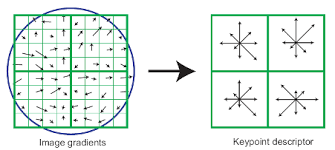
\includegraphics[width=0.7\linewidth]{figures/SIFTdescriptor}
	\caption{Descritor SIFT. As setas designam a soma dos gradientes nas caixas individuais. O círculo azul representa a região que é considerada na atuação do filtro Gausiano. Este exemplo ilustra uma matriz 8x8 resultando num 2x2 descritor. \cite{VisualOdometryRodasVehicles}}
	\label{fig:siftdescriptor}
\end{figure}

\subsection{SURF}

Uma janela quadrada é centrada no ponto de característica, com a mesma orientação. O tamanho da janela é 20\textit{s} x 20\textit{s} , onde \textit{s} é a escala onde o ponto característico foi detetado. De seguida, a janela é dividida em sub-regiões 4 x 4 . As respostas das ondas de Haar e seu valor absoluto são resumidas para direção horizontal e vertical em cada sub região. O descritor resultante consiste em um vetor 4D que contém as quatro somas para cada sub-região.


\section{Associação de Características}

O processo de correspondência de características é um requisito para muitas aplicações relacionadas com imagens, tais como, recuperação de uma imagem, deteção do movimento e reconstrução da forma. 
Como mencionado no início da Secção ~\ref{detCar}, espera-se que uma boa característica tenha como propriedade a diferenciabilidade. A diferenciabilidade permite que a característica seja identificada (idealmente) de maneira única.
As diferentes características determinadas pela etapa anterior precisam ser correspondidas, ou seja, é preciso determinar quais características são as mesmas em imagens distintas. Geralmente existem dois métodos diferentes para encontrar suas correspondências: correspondência de características e seguimento de características. 


\subsection{Correspondência de Características}

O método de correspondência de características consiste na deteção de características de maneira independente em todas as imagens com um determinado detetor de características.
Idealmente, as correspondências detetadas representam a mesma informação nas imagens.
Depois são efetuadas as correspondências entre as características detetadas usando uma estratégia de comparação baseada em medidas de semelhança.
Este método é muito usado em ambientes exteriores de grandes dimensões, em que as imagens são capturadas partir de posições distantes entre si, com a finalidade de limitar os problemas relacionados com desvio de movimento.

\subsubsection{Brute force}\label{subchap:BRUTE}

O método \textit{Brute force} compara um descritor de um conjunto de pontos caracteristicos da primeira image com todos os descritores dos pontos caracteristicos da segunda imagem. Geralmente, o descritor com pequena distância Euclidiana é comparado com o descritor da primeira imagem. A distância do descritor é limitada por um threshold de forma a tornar a comparação válida. O tempo entre duas imagens devem ser pequenas de forma à comparação do descritor ser correta.


\subsection{Seguimento de Características}

O método de seguimento de características, com alternativa, deteta características em apenas uma imagem com um determinado detetor de características. Na próxima imagem a característica correspondente é procurada na área em torno da localização da característica detetada.
Este método de deteção e seguimento é muito usado em ambientes interiores de pequenas dimensões e é adequado para aplicações de OV. 
Uma vez que as imagens são capturadas a partir de posições próximas e a quantidade de movimentos entre imagens sucessivas geralmente é pequena. 

\subsubsection{FLANN}\label{subchap:FLANN}

O método FLANN (do inglês, \textit{Fast Library for Approximate Nearest Neighbours}) é considerado um algoritmo que procura correspondência dos descritores numa vizinhança próxima do ponto característico.  O OpenCV utiliza uma correspondência baseada no FLANN que utiliza a estrutura de dados da árvore k-d e vizinhos próximos. K-d significa \textit{k} dimensões, onde \textit{k} é um inteiro positivo. A ideia base é :
\begin{itemize}
	\item Escolher uma dimensão \textit{k}.
	\item Encontrar o valor mediano dessa dimensão.
	\item Dividir a dimensão em duas partes com base no valor mediano.
	\item Repetir, até k-1 atingir 0 e começar de novo com k original até que todos elementos no conjunto de dados sejam examinados.
\end{itemize}

O processo é ilustrado na figura ~\ref{fig:flann} . Este exemplo inicia-se no ponto (7,2).

\begin{figure}[h!] %colocar figura a seguir ao texto anterior
	\begin{center}
		\leavevmode		
		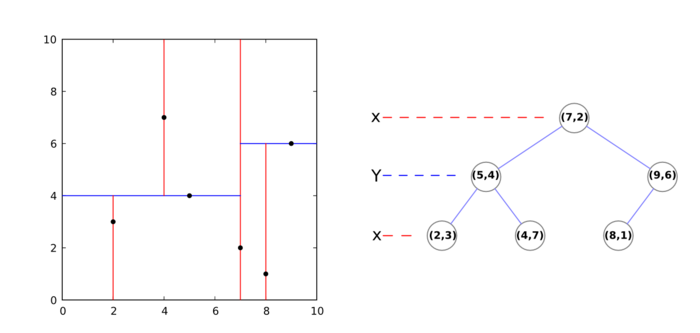
\includegraphics[width=0.8\textwidth]{flann}
		\caption{A imagem da esquerda ilustra a decomposição 2-d, note que as linhas vermelhas são para o eixo x e as linhas azuis para o eixo y. A imagem da direita ilustra a árvore 2-d correspondente.}
		\label{fig:flann}
	\end{center}
\end{figure}

Uma vez que a árvore k-d é formada, o próximo passo é usar pontos do segundo conjunto de dados e ver em qual nó da árvore k-d que o ponto examinado está mais próximo. O procedimento é chamado vizinho mais próximo (NN, do inglês, \textit{Nearest Neighbour}). Começando no nó raiz (7,2), como ilustrado, o algoritmo percorre a árvore 2-d construída recursivamente. Escolhe o nó da esquerda ou direita se o ponto examinado tiver um valor maior ou menos que o nó atual na dimensão atual, respetivamente. Uma vez que o algoritmo tenha atingido um nó final, o algoritmo guarda esse nó como o melhor atualmente. A recursão é então finalizada e o algoritmo começa a atravessar de volta ao nó raiz. A distância até ao ponto examinado é verificada em cada nó, se a distância for menor então é atualizado o melhor valor. O algoritmo também verifica se o hiperplano do outro lado da árvore está dentro do raio da menor distância atual, se não , esse hiperplano é descartado. Se estiver dentro, o algoritmo percorre esse ramo da árvore k-d também. O procedimento pode ser visto na figura ilustrada ~\ref{fig:flannNN}.

\begin{figure}[h!] %colocar figura a seguir ao texto anterior
	\begin{center}
		\leavevmode		
		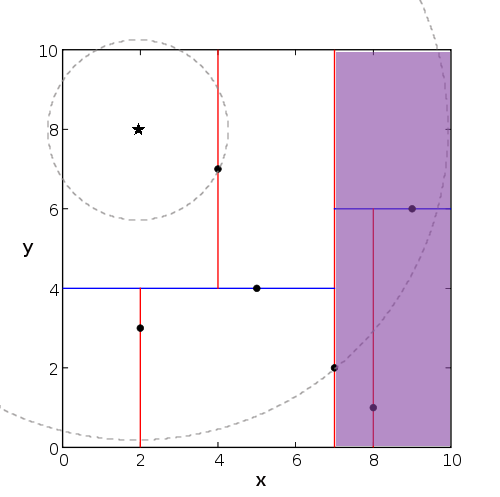
\includegraphics[width=0.6\textwidth]{flannNN}
		\caption{Algoritmo de procura NN baseado nas árvores 2-d.}
		\label{fig:flannNN}
	\end{center}
\end{figure}

O ponto (2,8) é examinado para o seu vizinho mais próximo, marcado com uma estrela na figura. O algoritmo começa no nó raiz (7,2) e a distância , isto é , o raio do grande circulo centrado na estrela cobre todos os hiperplanos. Isso significa que não podemos descartar nenhum hiperplano. O algoritmo percorre a árvore, ignorando os hiperplanos roxos da figura. O nó da folha (4,7) é definido como o melhor e o algoritmo começa a atravessar de volta para o nó raiz, verificando a distância em cada nó. Desde que o raio do pequeno círculo centrado em torno da estrela é a melhor combinação atual e não está se cruzando com os hiperplanos roxos, pode-se descartar esses hiperplanos e o algoritmo não procura por eles. Uma vez no nó raiz, o algoritmo termina e (4,7) era de fato o mais próximo vizinho.

\section{Estimação do movimento}

A etapa de estimação do movimento representa o núcleo da computação em um sistema de OV. Ela efetua o cálculo do movimento da câmara entre a imagem atual e a imagem anterior. A trajetória da câmara e do agente (assumindo que estão ligados rigidamente) pode ser recuperada completamente através da concatenação de todos os movimentos individuais.

Esta secção explica com a transformação relativa \textit{$T_k$} pode ser calculada entre duas imagens \textit{$I_{k-1}$} e \textit{$I_k$} a partir de dois conjuntos de pontos característicos correspondentes \textit{$f_{k-1}$} , \textit{$f_k$} nos instantes de tempo \textit{k - 1} e \textit{k}, respetivamente. Existem três métodos diferentes para o cálculo do \textit{$T_k$} dependendo se as correspondências dos pontos característicos são especificadas em três ou duas dimensões. Os métodos referidos são:


\begin{itemize}
	\item 2D-para-2D: Neste caso, ambos \textit{$f_{k-1}$} e \textit{$f_k$} são especificados pelas coordenadas 2D da imagem.
	\item 3D-para-3D: Neste caso, ambos \textit{$f_{k-1}$} e \textit{$f_k$} são especificados pelas coordenadas 3D da imagem. Para realizar esta acção, é necessário a triangulação de pontos 3D em cada instante de tempo, isto pode ser feito a partir de um sistema com câmaras estéreo, por exemplo.
	\item 3D-para-2D: Neste caso, \textit{$f_{k-1}$} são especificados em 3D e \textit{$f_k$} são as suas correspondentes reprojeções em 2D na imagem \textit{$I_k$}.No caso da utilização de um sistema monocular, a estrutura 3D necessita de triangular duas câmaras adjacentes (isto é \textit{$I_{k-2}$} e \textit{$I_{k-1}$}) e assim a construção da imagem 2D . 
\end{itemize}



\subsection{2D-para-2D}

A relação geométrica entre duas imagens \textit{$I_k$} e \textit{$I_{k-1}$} da calibração da câmara é descrita pela matriz essencial \textit{E}. Esta contém os parâmetros de movimento da câmara para um fator de escala desconhecido. \[ E_k\ \approx\ {\hat{t}}_kR_k \] onde \textit{$t_k$} = $[ \textit{$t_x$}, \textit{$t_y$}, \textit{$t_z$} ]^T$ e \[ \hat{t}_k =\ \left[\begin{array}{ccc}0&-t_z&t_y\\t_z&0&-t_x\\-t_y&t_x&0\\\end{array}\right] . \]

A correspondência dos pontos característico, rotações e translações podem ser obtidos através da matriz essencial. A principal propriedade da estimação de movimento através de 2D-para-2D é a restrição epipolar, que determina a linha em cada ponto de característica correspondente em outra imagem, como ilustrado na Figura ~\ref{fig:epipolarconstrait}.

\begin{figure}[h!]
	\centering
	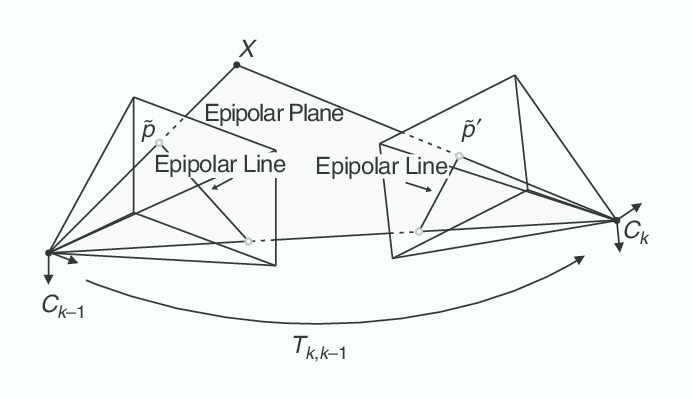
\includegraphics[width=0.7\linewidth]{figures/equipolarline}
	\caption{Uma ilustração da restrição epipolar. \cite{VOpart1}}
	\label{fig:epipolarconstrait}
\end{figure}

Esta restrição pode ser formulada por $p'^{T}$Ep = 0, onde p é um ponto característico numa imagem e $p'$ é o correspondente ponto característico noutra imagem.

Através da estimação da matriz \textit{E}, a rotação e translação pode ser extraída. 
\[ R = U(\pm W^T)V^T ,\] \[ \hat{t} =  U(\pm W)SU^T, \] 
onde \[  W^T = \left[\begin{array}{ccc}0&\pm1&0\\\mp1&0&0\\0&0&1\\\end{array}\right] \] 
e U, S, V são obtidas através do USV (do inglês, \textit{Singular Value Decomposityon}) \[ E = USV^T \]

Para recuperar a trajetória de uma sequência de imagens é necessário a concatenação das diferentes transformações \textit{$T_{0:n}$}. Para isso é necessário uma escala relativa obtida através de : \[ r = \frac{ \| X_{k-1,i} - X_{k-1,j} \| }{ \| X_{k,i} - X_{k,j} \| } \] 

Desta forma, o algoritmo de OV com correspondência 2D-para-2D é sumariado de seguida:
\begin{enumerate}
	\item Capturar uma imagem \textit{$I_{k}$}.
	\item Extrair e conjugar pontos característicos entre \textit{$I_{k-1}$} e \textit{$I_{k}$}.
	\item Obter a matriz essencial do par de imagens \textit{$I_{k-1},I_k$}.
	\item Decompor a matriz essencial em \textit{$R_k$} e \textit{$\hat{t}_k$}.
	\item Computorizar a escala relativa \textit{$\hat{t}_k$}.
	\item Concatenar a transformação $C_k$ = $C_{k-1}$ $T_k$.
	\item Repetir 1.
\end{enumerate}


\subsection{3D-para-3D}

A estimação do movimento através da correspondência 3D-para-3D é usada em sistemas estéreo. 

A solução geral é encontrar \textit{$T_k$} que minimiza a distância \textit{$L_2$} entre duas 3D características \[ \arg_{\ T_k}^{min}\sum_{i}{\left \| \tilde{X}_k^i - T_k\tilde{X}_{k-1}^i \right \|} \] 
onde \textit{i} é a característica \textit{i} e \textit{$X_{k},X_{k-1}$} são as coordenadas homogéneas dos pontos 3D. 

Como analisado anteriormente, o número mínimo de soluções são três correspondências não colineares. Desta forma, se n $\geq$ 3, uma solução possível é realizar a diferença dos centroides das características 3D e uma rotação usando SVD. A translação é dada por \[ t_{k\ }=\ {\bar{X}}_k\ -\ R{\bar{X}}_{k-1} \] onde - é a média aritmética.

A rotação é eficientemente calculada através do SVD como \[ R_k = VU^T \] onde $USV^T$ = $svd({(X_{k-1}\ -\ {\bar{X}}_{k-1})(X_k\ -\ {\bar{X}}_k)}^T)$ e \textit{$X_k$} corresponde ao ponto 3D.

O algoritmo de OV com correspondência 3D-para-3D é sumariado de seguida:
\begin{enumerate}
	\item Capturar duas pares de imagens num sistema estéreo, \textit{$I_{l,k-1}$},\textit{$I_{r,k-1}$} e \textit{$I_{l,k}$},\textit{$I_{r,k}$}
	\item Extrair e conjugar pontos característicos entre \textit{$I_{l,k-1}$} e \textit{$I_{l,k}$}
	\item Triangular os pontos característicos conjugados para cada par de estéreo.
	\item Computacional \textit{$T_k$} de pontos característicos 3D, \textit{$X_{k-1}$} e \textit{$X_k$}  
	\item Concatenar a transformação $C_k$ = $ C_{k-1}$ $T_k$
	\item Repetir 1
\end{enumerate}



\subsection{3D-para-2D}

A estimação do movimento de 3D-para-2D é mais precisa do que 3D-para-3D porque são minimizados os erros de reprojeção. A transformação \textit{$T_k$} é analisada num sistema estéreo através do \textit{$X_{k-1}$} e \textit{$p_k$}. No caso de um sistema monocular, através da triangulação das medições de imagens \textit{$p_{k-1}$} e \textit{$p_{k-2}$}. 

A formula general neste caso é encontrar \textit{$T_k$} que minimize o erro de reprojeção da imagem \[ \arg_{\ T_k}^{min} \sum_{i}{\left \| p_k^i - \hat{p}_{k-1}^i \right \|}^2 \]
onde \textit{$p_{k-1}$} é a reprojeção do ponto 3D \textit{$X_{k-1}^i$} na imagem \textit{$I_k$} de acordo com a transformação \textit{$T_k$}. 

Como no problema da correspondência 3D-para-3D são necessários um número mínimo de pontos. Com um número de pontos igual a 6, P é calculado através do uso de SVD e a rotação e translação é obtida através de $P_k$ = [R|t]. 

Assim, a estimação através de 3D-para-2D assume que os pontos são obtidos de apenas uma câmara. Desta forma, num sistema estéreo o ponto 2D é obtido através da junção da câmara da esquerda com a câmara da direita. Obviamente a captura das imagens têm de ser no mesmo instante de tempo.  Para o caso de um sistema monocular é algoritmo inicializa após a captura das duas primeiras imagens, desta forma é necessário triangular duas imagens capturadas em instantes diferentes para obter o ponto.

O algoritmo de OV com correspondência 3D-para-2D é sumariado de seguida:
\begin{enumerate}
	\item Realizar na primeira vez:
	\begin{enumerate}[label*=\arabic*.]
		\item Capturar duas imagens \textit{$I_{k-2}$},\textit{$I_{k-1}$} 
		\item Extrair e conjugar pontos característicos entre eles
		\item Triangular os pontos característicos \textit{$I_{k-2},I_{k-1}$}
	\end{enumerate}
	\item Realizar a cada iteração:
	\begin{enumerate}[label*=\arabic*.]
		\item Capturar nova imagem \textit{$I_k$}
		\item Extrair e conjugar pontos característicos com a imagem anterior \textit{$I_{k-1}$}
		\item Computorizar posição da câmara através do calculo 3D-para-2D
		\item Triangular todos os novos pontos característicos entre \textit{$I_k$} e \textit{$I_{k-1}$}
		\item Repetir 2.1
	\end{enumerate}
	
\end{enumerate}




\section{Métodos de ajuste de erros}

A associação de pontos , usualmente, está contaminada por \textit{outliers}\footnote{valor atípico, é uma observação que apresenta um grande afastamento das demais series ou é inconsistente.}, isto é, associação de dados errada. As possíveis causas de \textit{outliers} são ruídos da imagem, exclusões, pouca nitidez, alteração de posições e iluminação das quais os modelos matemáticos dos detetores de características não detetam. 

Para  a estimação da movimentação correta da câmara é importante que o \textit{outliers} sejam removidos. 

\subsection{Windowed bundle adjustment}

O \textit{bundle adjustment} é um algoritmo criado no campo da fotometria em meados da década de 1950 e tornou-se muito utilizado no campo da visão por computador, explicitamente na área de reconstrução 3D.

A função principal é tentar otimizar ao mesmo tempo os parâmetros (intrínsecos e extrínsecos) da câmara, bem como os parâmetros dos pontos 3D de referência. Ele é aplicado para os casos em que as características detetadas numa imagem são procuradas em mais do que duas características. Este algoritmo considera uma "janela" de \textit{n} características da imagem e depois faz uma otimização dos parâmetros das posições da câmara e dos pontos 3D de referência para este conjunto de características da imagem.

No \textit{bundle adjustment}, a função de erro a minimizar é o erro de reprojeção da imagem. 
\[ \arg_{X^i,C_k}^{min} \sum_{i,k}{\left \| p_k^i - g(X^i ,C_k) \right \|}^2 ,\]
onde $p_k^i$ é o i-ésimo ponto da imagem dos pontos 3D de referência \textit{$X^1$} medido na k-ésima imagem e $\textit{g}(X^i,C_k)$ é a sua imagem de reprojeção de acordo com a posição atual da câmara $C_k$. O erro de reprojeção é uma função não-linear.

Para concluir, o principal objetivo do \textit{bundle adjustment} em sistemas de OV é a redução do desvio entre a trajetória estimada e a real.

\subsection{RANSAC}


Tal como referido anteriormente, uma das funções do algoritmo RANSAC é a remoção dos \textit{outliers}, que permite a estimação do movimento da câmara de uma forma mais precisa. A etapa de rejeição dos \textit{outliers} é a mais delicada em sistema de OV.

De uma forma geral, este algoritmo é utilizado quando se pretende estimar um modelo (por exemplo os parâmetros de rotação e translação de uma câmara) na presença de \textit{outliers}.

A ideia fundamental do RANSAC é calcular candidatos modelo a partir de amostras de conjuntos de pontos de dados. A escolha das amostras é feita aleatoriamente. Posteriormente com os outros dados é selecionada como solução.

O esboço deste algoritmo é apresentado em seguida:

%%Inserir figura de algoritmo

O número de iterações N necessário para garantir a solução correta é calculado pela equação

\[  N = \frac{log(1-p)}{log(1-(1-\epsilon)^s)} \]

O valor \textit{s} representa o número de pontos de dados a partir do qual o modelo pode ser instanciado, $\epsilon$ é a percentagem de \textit{outliers} nos pontos de dados e \textit{p} representa a probabilidade de sucesso pretendida.

Notar que o algoritmo é um método iterativo e não determinístico de tal forma que calcula uma diferente solução em cada execução. Contudo, a solução tende a estabilizar à medida que o número de iterações aumenta.
